予測モデルを入力$x$, パラメタ$\Theta$として
\begin{eqnarray*}
    y=f(x;\Theta)
\end{eqnarray*}
と表す.\\
このとき予測モデルの入力は説明変数(explanatory variable), 独立変数(independent variable), 予測変数(predictor)に分類され, それに応じて出力$y$は目的変数(objective variable), 従属変数(dependent variable), 応答変数(response variable)となる. \\
たとえば, 予測モデル$y=f(x;\Theta)$に対して,
\begin{eqnarray*}
    y=ax+b,\ \ \Theta = (a,b)
\end{eqnarray*}
とおくと予測モデルは次のようになる.
\begin{center}
    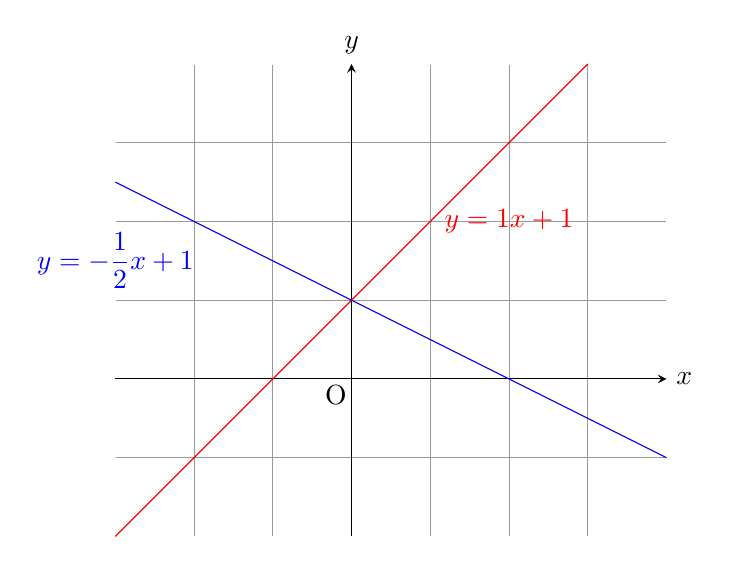
\begin{tikzpicture}[>=stealth]
        \draw[draw=gray!80] (-2.99,-1.99) grid (3.99,3.99);
        \draw[->] (-3,0)--(4,0) node[right] {$x$};
        \draw[->] (0,-2)--(0,4) node[above] {$y$};
        \node at(-0.2,-0.2) {O};
        \draw[draw=red,domain=-3:3] plot(\x,{\x+1});
        \draw[draw=blue,domain=-3:4] plot(\x,{-0.5*\x+1});
        \node at(2,2) {\textcolor{red}{$y=1x+1$}};
        \node at(-3,1.5) {\textcolor{blue}{$\displaystyle y=-\frac{1}{2}x+1$}};
    \end{tikzpicture}
\end{center}
この場合の$y$は量的データのときの予測問題であり\textcolor{red}{回帰(regression)}と呼ぶ.\\
また,
\begin{eqnarray*}
    y={\rm sgn}(ax+b),\ \ \Theta(a,b)
\end{eqnarray*}
とおくと予測モデルは次のようになる.
\begin{center}
    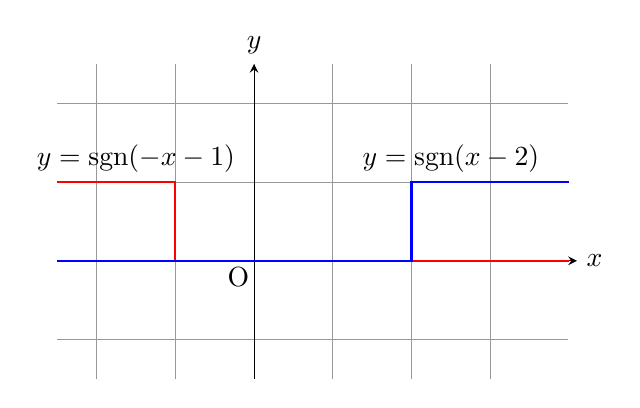
\begin{tikzpicture}[>=stealth]
        \draw[draw=gray!80] (-2.5,-1.5) grid (3.99,2.5);
        \draw[->] (-2.5,0)--(4.1,0) node[right] {$x$};
        \draw[->] (0,-1.5)--(0,2.5) node[above] {$y$};
        \node at(-0.2,-0.2) {O};
        \draw[draw=red,thick] (-2.5,1)--(-1,1)--(-1,0)--(4,0);
        \draw[draw=blue,thick] (-2.5,0)--(2,0)--(2,1)--(4,1);
        \node at(-1.5,1.3) {$y={\rm sgn}(-x-1)$};
        \node at(2.5,1.3) {$y={\rm sgn}(x-2)$};
    \end{tikzpicture}
\end{center}
この場合の$y$の質的データのときの予測問題であり\textcolor{red}{分類/識別(Classification)}と呼ぶ. 質的データとはカテゴリ, 離散データ, クラスといったものである. 大人を1, 小人を0として人数を分類したものも質的データにあたる.